%%%%%%%%%%%%%%%%%%%%%%%%%%%%%%%%%%%%%%%%%%%%%%%%%%%%
%%%%%%%%%%%%%%%%%%%%%%%%%%%%%%%%%%%%%%%%%%%%%%%%%%%%
% Chapitre 3
\chapter{Intégration de l'IA Générative dans les Systèmes de Recommandation Éducatifs}

% Introduction du chapitre
\section*{Introduction}
\phantomsection
\addcontentsline{toc}{section}{Introduction}

\paragraph{}
La sélection des cours constitue un élément essentiel du parcours universitaire de tout étudiant, influençant profondément son expérience académique ainsi que ses perspectives professionnelles futures \cite{BruchFeinberg2017}. Au sein des facultés marocaines, notamment dans les grandes universités publiques telles que celles de Rabat, Casablanca ou Marrakech, où des milliers de modules sont proposés chaque année, ce processus peut devenir complexe et long, surtout pour les étudiants nouvellement inscrits.

\paragraph{}
Traditionnellement, les étudiants marocains s’orientent à l’aide des conseils des enseignants, des responsables pédagogiques, ou en se basant sur les expériences partagées par leurs camarades. Cependant, cette méthode peut générer des inégalités dans l’accès à une information fiable et complète, puisque tous les étudiants ne bénéficient pas du même accompagnement ni du même réseau de contacts informés \cite{LynchORiordan1998}.

\paragraph{}
Dans d’autres domaines, les systèmes de recommandation comme le filtrage collaboratif ont été utilisés avec succès pour offrir des suggestions personnalisées. Néanmoins, lorsqu’il s’agit de recommander des cours universitaires dans le contexte de l’enseignement supérieur marocain, ces systèmes se heurtent à plusieurs limitations, notamment l’absence de données structurées, la diversité des filières, et le manque de retour systématique sur les performances des modules.

% Contexte général
\section*{Contexte de l’utilisation de l’intelligence artificielle générative dans l’éducation}
\addcontentsline{toc}{section}{Contexte de l’IAG}

\paragraph{}
L’intelligence artificielle générative (IAG), représentée par des modèles comme \textit{GPT} (Generative Pre-trained Transformer), \textit{BERT} ou encore \textit{LLaMA}, marque une nouvelle ère dans le domaine de l’intelligence artificielle. Contrairement aux systèmes traditionnels de traitement de l’information, ces modèles sont capables de générer de manière autonome des textes cohérents, de répondre à des questions, de résumer des documents, ou encore de produire du contenu personnalisé. Ces capacités ont rapidement attiré l’attention du secteur éducatif, en quête de solutions innovantes pour améliorer l’apprentissage et l’accompagnement pédagogique.

\paragraph{}
Dans un contexte où les apprenants sont de plus en plus nombreux, diversifiés et connectés, les établissements éducatifs sont confrontés à des défis majeurs : comment personnaliser l’enseignement, soutenir les élèves en difficulté, fournir un accès équitable au savoir et répondre aux attentes d’une génération numérique ? L’IAG apparaît comme une réponse prometteuse à ces problématiques.

\paragraph{}
Par exemple, les outils basés sur l’IAG peuvent générer des exercices adaptés au niveau d’un élève, résumer un cours long en quelques phrases clés, ou encore simuler un échange interactif avec un tuteur virtuel. Plus encore, l’IA générative permet de créer des parcours d’apprentissage personnalisés, d’analyser les productions des élèves pour fournir un retour immédiat et intelligent, ou de recommander des ressources en fonction du style d’apprentissage de chacun.

\paragraph{}
Cependant, cette technologie suscite aussi des interrogations : peut-elle vraiment remplacer l’accompagnement humain ? Est-elle capable de respecter la diversité des contextes pédagogiques ? Quels sont les risques d’un usage non encadré (biais, erreurs, plagiat) ?

\paragraph{}
Dans ce contexte, l’intégration de l’intelligence artificielle générative dans les systèmes éducatifs doit être pensée avec rigueur, en tenant compte à la fois de ses potentialités et de ses limites. Ce chapitre se propose d’explorer les contributions spécifiques de l’IAG dans le cadre des systèmes de recommandation éducatifs, en mettant en lumière ses applications concrètes, ses mécanismes techniques, ainsi que les défis qu’elle soulève.

% Objectifs du chapitre
\section*{Objectifs du chapitre}
\addcontentsline{toc}{section}{Objectifs du chapitre}

Ce chapitre vise à :

\begin{itemize}
  \item Présenter le contexte général de l’émergence de l’intelligence artificielle générative (IAG) et son évolution récente ;
  \item Expliquer les principes de fonctionnement des modèles génératifs comme \textit{GPT}, \textit{BERT}, ou \textit{LLaMA} ;
  \item Identifier les opportunités offertes par l’IAG dans le domaine de l’éducation, en particulier en matière de personnalisation de l’apprentissage ;
  \item Illustrer les cas d’usage concrets de l’IAG dans les systèmes éducatifs, notamment dans les systèmes de recommandation pédagogique ;
  \item Mettre en évidence les limites, risques et défis éthiques associés à l’usage de l’IAG dans l’enseignement ;
  \item Fournir une base de réflexion pour une intégration responsable et efficace de l’IAG dans les environnements d’apprentissage.
\end{itemize}

% Rôle des LLM
\section*{Rôle des modèles de type LLM (Large Language Models)}
\addcontentsline{toc}{section}{Rôle des LLM}

\paragraph{}
Les modèles de langage de grande taille (\textit{Large Language Models}, LLM) sont au cœur des avancées récentes en intelligence artificielle générative. Ces modèles, entraînés sur des corpus massifs de textes, sont capables de comprendre, générer et transformer du langage naturel avec un niveau de fluidité et de pertinence sans précédent.

Dans le contexte éducatif, les LLM jouent plusieurs rôles essentiels :

\begin{itemize}
    \item \textbf{Génération de contenu pédagogique :} production automatique de supports de cours, d’exercices, d’explications détaillées ou de résumés adaptés ;
    \item \textbf{Personnalisation de l’apprentissage :} recommandation de ressources spécifiques, adaptation de la difficulté, propositions de parcours individualisés ;
    \item \textbf{Assistance interactive :} réponses aux questions des étudiants via des chatbots éducatifs ;
    \item \textbf{Analyse des productions :} évaluation automatique des rédactions, retour pédagogique immédiat.
\end{itemize}

\paragraph{}
Toutefois, l’efficacité des LLM dépend fortement de la qualité des données d’entraînement et de leur contextualisation. Leur rôle est de compléter l’enseignement, non de le remplacer.

% Apports de l’IAG
\section{Apports de l’IA générative aux systèmes de recommandation éducatifs}

L’intelligence artificielle générative (IAG) transforme en profondeur les systèmes de recommandation éducatifs, en dépassant les approches classiques fondées uniquement sur des filtrages collaboratifs ou des modèles statistiques. Grâce à sa capacité à comprendre, générer et adapter des contenus pédagogiques en langage naturel, l’IAG permet de concevoir des systèmes plus intelligents, plus adaptatifs et véritablement centrés sur les besoins individuels des apprenants.

\subsection{Personnalisation avancée des parcours d’apprentissage}

L’un des principaux apports de l’IA générative réside dans sa capacité à analyser des données complexes liées aux apprenants : préférences personnelles, style cognitif, historique des performances, interactions avec la plateforme, etc. Ces informations permettent de construire des profils d’apprentissage détaillés et dynamiques.

\paragraph{} Ainsi, le système peut recommander des séquences pédagogiques personnalisées. Par exemple, un étudiant en difficulté sur un chapitre donné se verra proposer des modules de renforcement ciblés, tandis qu’un autre, plus avancé, sera orienté vers des contenus plus exigeants. Cette personnalisation évolue en temps réel selon la progression et l’engagement de l’apprenant, ce qui améliore l’efficacité de l’apprentissage.

\subsection{Génération de contenus pédagogiques adaptés}

Contrairement aux approches traditionnelles, l’IAG est capable de générer automatiquement du contenu éducatif pertinent et personnalisé. Ces contenus incluent notamment :

\begin{itemize}
  \item des exercices adaptés au niveau de l’élève ;
  \item des quiz d’auto-évaluation dynamiques ;
  \item des résumés intelligents de leçons ou de chapitres ;
  \item des explications alternatives ou simplifiées en fonction du style d’apprentissage.
\end{itemize}

\paragraph{} Cette production automatisée représente un gain de temps considérable pour les enseignants, tout en offrant aux élèves une diversité de supports et une meilleure accessibilité aux connaissances. Le contenu généré est aussi actualisable en fonction du niveau et du rythme de chaque apprenant.

\subsection{Réponses contextuelles et interactives aux besoins des apprenants}

Les modèles de langage avancés (comme GPT) permettent aux systèmes éducatifs d’interagir avec les utilisateurs en langage naturel. Ils peuvent :

\begin{itemize}
  \item répondre à des questions de manière contextuelle et instantanée ;
  \item fournir des éclaircissements supplémentaires sur une notion ;
  \item guider l’élève dans la résolution d’un problème ou d’un exercice, étape par étape.
\end{itemize}

\paragraph{} 
Ces interactions enrichissent considérablement l’expérience d’apprentissage en la rendant plus fluide, plus engageante et mieux adaptée aux besoins ponctuels des apprenants. Le système joue ainsi un rôle d’accompagnateur pédagogique intelligent, disponible à tout moment.

\section{Systèmes à base de connaissances}
\paragraph{} 
Pour surmonter les limitations du démarrage à froid, certains chercheurs ont développé des systèmes de recommandation à base de connaissances qui intègrent une expertise du domaine et des règles académiques. Par exemple, CrsRecs (Ng et Linn, 2017) utilise l'analyse de sujets, l'analyse des sentiments et des données d'enquêtes sur les priorités des étudiants pour classer les cours potentiels. Ces systèmes peuvent formuler des recommandations même sans disposer de nombreuses données historiques, mais nécessitent un effort considérable pour encoder les connaissances du domaine et les règles.

\section{Approches hybrides}
\paragraph{} 
Des travaux récents se sont concentrés sur des approches hybrides combinant plusieurs techniques de recommandation. Pathways (Chen et al., 2022) visualise les tendances d’inscription aux cours dans le passé tout en prenant en compte les intérêts des étudiants et les exigences académiques. Le système aide les étudiants à explorer les différentes options de cours via une interface interactive, en équilibrant la personnalisation et la découverte fortuite. De même, Salehudin et al. (2019) proposent un modèle de filtrage collaboratif qui s’intègre aux tendances historiques d’inscription ainsi qu’aux données de performance des étudiants afin de fournir des recommandations personnalisées.

\section{Exigences en matière de données}
\paragraph{} 
La plupart des approches de recommandation avancées nécessitent une collecte de données étendue sur plusieurs semestres ou années académiques pour construire des modèles efficaces (Salehudin et al., 2019). Cette exigence représente un défi pour les établissements souhaitant mettre en place de tels systèmes, car ils doivent consacrer beaucoup de temps à identifier les sources de données et à organiser l’accès aux informations réparties sur plusieurs serveurs, souvent gérés par différentes unités, avant que le système ne devienne réellement utile.

Les universités sont des environnements où les données s’échappent facilement, et les acteurs privés peuvent bénéficier d’un avantage s’ils parviennent à agréger des données fournies par les étudiants eux-mêmes, issues de plusieurs établissements. Les dirigeants universitaires doivent se préparer en interne avant que des solutions externes de recommandation de cours ne fassent leur apparition sur leur campus. Le travail présenté ici reflète une philosophie de prise en main et de développement innovant de l’environnement informationnel et décisionnel de l’institution.


\section{LLM pour les systèmes de recommandation}
\paragraph{} 
Les avancées récentes dans les modèles de langage de grande taille (LLM) ont ouvert de nouvelles perspectives pour les systèmes de recommandation. Plutôt que de considérer la recommandation comme un simple problème d’appariement ou de classement, les LLM permettent une approche plus souple en transformant les tâches de recommandation en problèmes de compréhension et de génération du langage (Geng et al., 2023). Cela permet aux systèmes de recommandation d’exploiter la compréhension sémantique riche et les capacités de génération des modèles linguistiques, tout en fournissant un cadre unifié pour diverses tâches de recommandation.

Les LLM peuvent remplir plusieurs rôles dans les systèmes de recommandation (Xu et al., 2024). Ils peuvent effectuer de l’ingénierie de caractéristiques en générant des descripteurs textuels riches, extraire des représentations sémantiques (embeddings) pour les éléments ou les utilisateurs afin de résoudre les scénarios de démarrage à froid, agir comme systèmes de recommandation directs, ou encore servir de contrôleurs pour permettre des recommandations plus interactives et explicables. Ces capacités peuvent être exploitées via des approches « zero-shot » ou « few-shot » à l’aide d’invites soigneusement conçues, ou encore par un ajustement (fine-tuning) sur des données de recommandation spécifiques au domaine.

L’un des avantages majeurs des systèmes de recommandation basés sur des modèles linguistiques est leur capacité à unifier divers types d’informations et de tâches dans un seul et même cadre. Comme le montre le système M6-Rec (Cui et al., 2022), un modèle fondamental unique peut prendre en charge plusieurs tâches de recommandation en les transformant en problèmes de compréhension et de génération du langage. Cela inclut des tâches classiques comme la recherche et le classement, ainsi que des tâches plus complexes comme la génération d’explications ou les recommandations conversationnelles. L’approche basée sur des représentations textuelles permet au système de traiter les données comportementales des utilisateurs, les métadonnées des éléments et les interactions utilisateur-élément dans un format cohérent, tout en contournant les limites des systèmes basés sur les identifiants lorsqu’il s’agit d’éléments jamais vus auparavant.

\section{Processus de Recommandation de Cours}
\paragraph{} 
Le système de recommandation de cours utilise une approche hybride combinant la recherche de similarité basée sur des \textit{embeddings} et le raisonnement d’un grand modèle de langage (LLM) afin de fournir des suggestions de cours personnalisées. Les utilisateurs interagissent avec le système de recommandation en utilisant un langage naturel pour décrire leur parcours, leurs centres d’intérêt et leurs objectifs. Le système fonctionne sur une base de données contenant des descriptions de cours et permet aux utilisateurs de restreindre l’espace de recherche grâce à un filtrage simple basé sur les niveaux des cours, ce qui permet d’obtenir des recommandations adaptées aux différents niveaux académiques.

Le processus de recommandation comprend cinq opérations principales illustrées dans la Figure~1 et organisées en deux étapes :

\begin{enumerate}
    \item \textbf{Génération de Contexte} : Création d’un contexte de recherche pertinent à partir de la requête de l’utilisateur
    \item \textbf{Recommandation} : Identification et classement des cours les plus adaptés
\end{enumerate}
\begin{minipage}{1\textwidth}
		\centering
		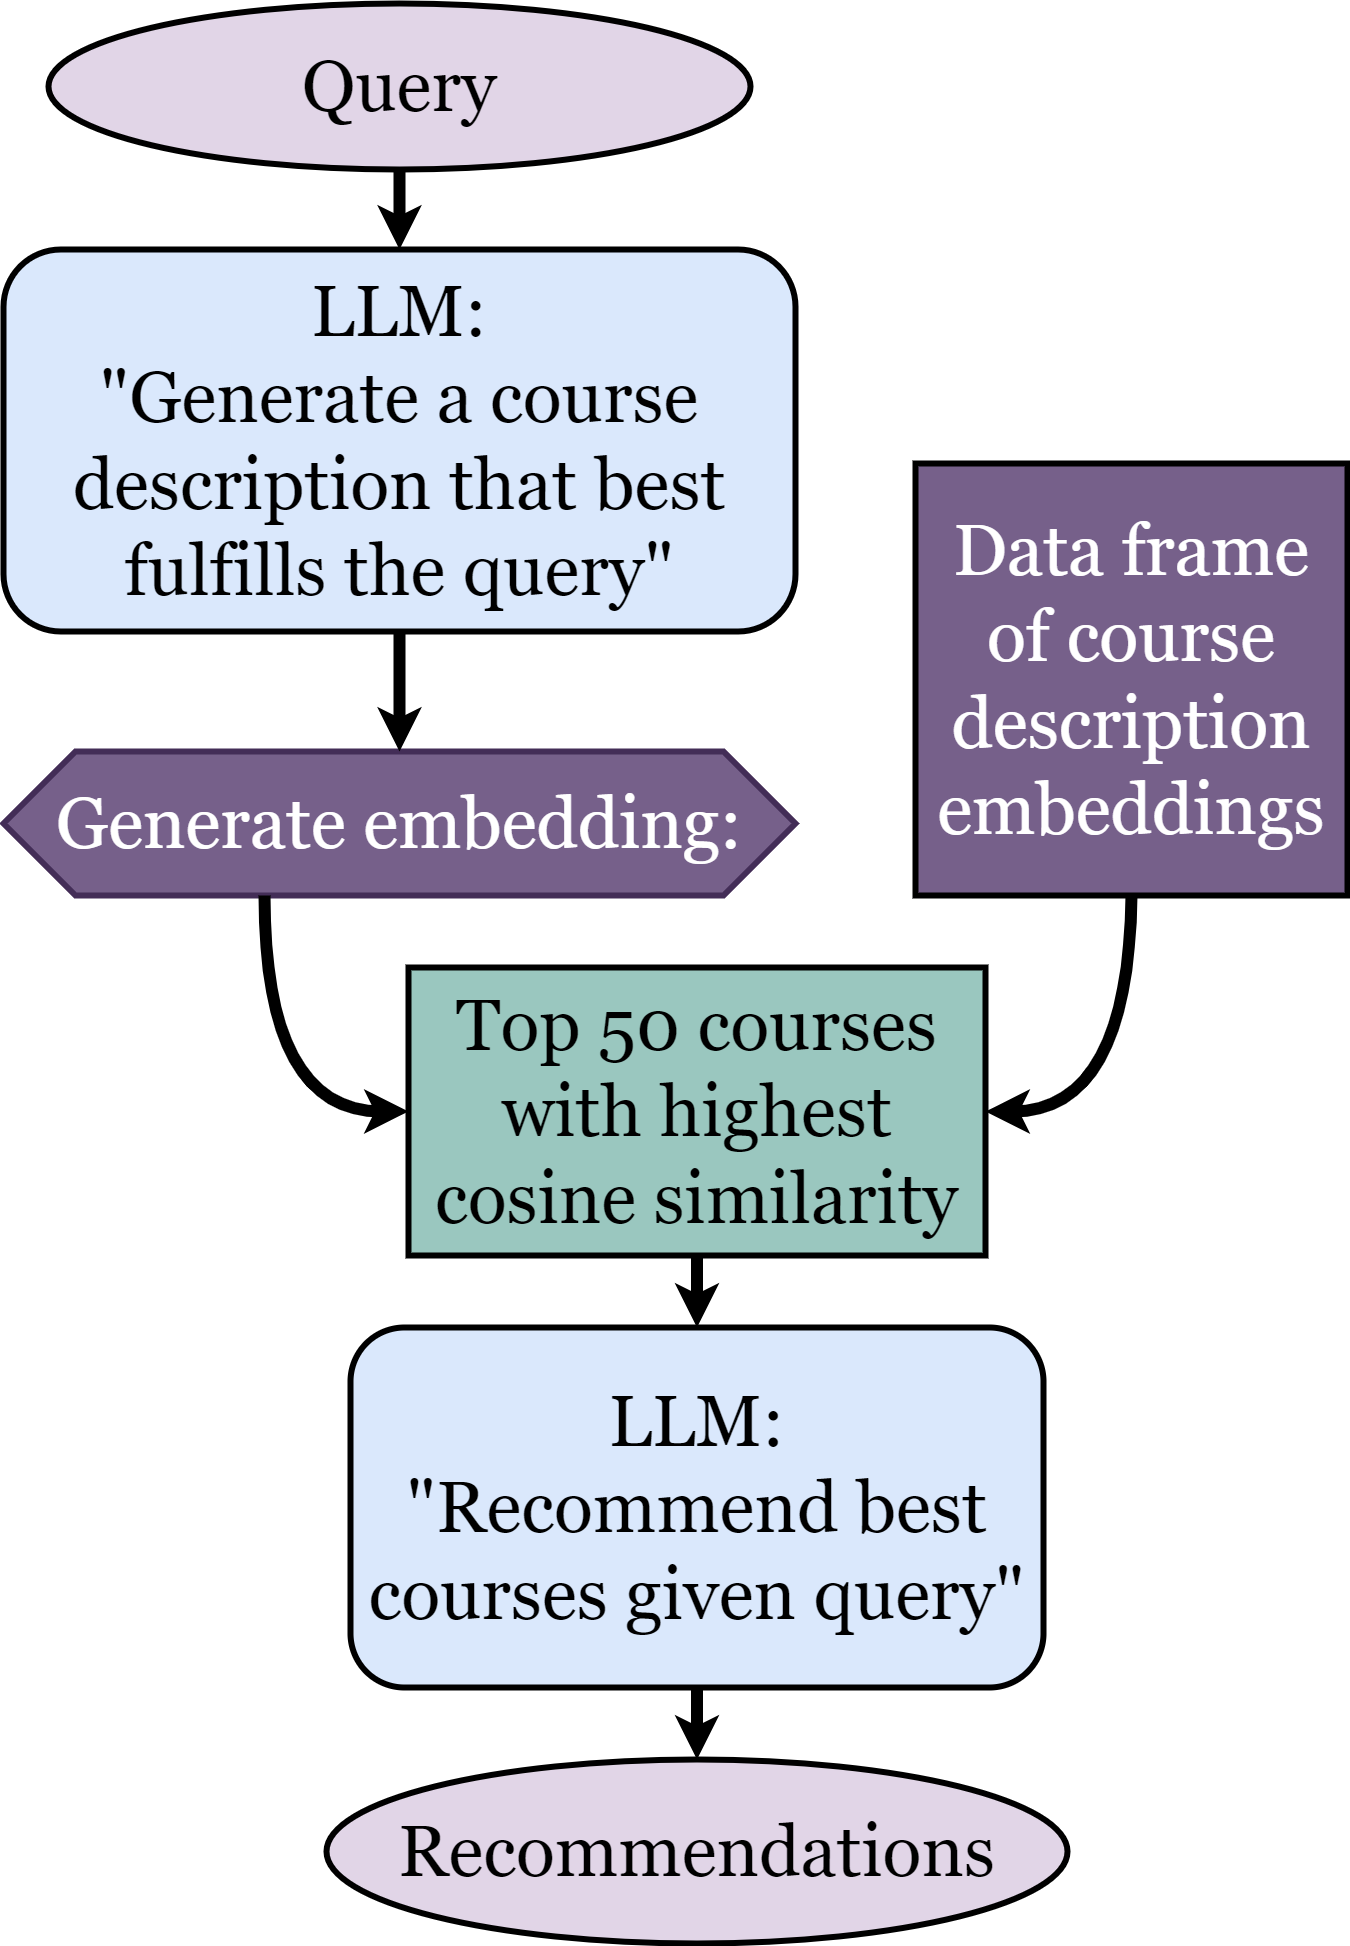
\includegraphics[width=\linewidth]{images/EmbRecommenderDiagram.png}
		\captionof{figure}{Pipeline hybride LLM-Embedding pour les recommandations de cours}
\end{minipage}
\section{Données}

Le système repose sur un \textbf{fichier CSV} contenant les informations descriptives des cours. Ces données sont chargées dans un \textbf{dataframe Pandas} pour traitement. Chaque enregistrement représente un cours et contient les champs suivants :

\begin{itemize}
    \item \textbf{Objectifs académiques visés} (Academic Goals)
    \item \textbf{Filière ou spécialisation concernée} (Major)
    \item \textbf{Loisirs liés au contenu du cours} (Hobbies)
    \item \textbf{Compétences informatiques requises ou développées} (Computer Skills)
    \item \textbf{Intérêt pour les langues} (Interest in Languages)
    \item \textbf{Moyenne générale minimale recommandée} (GPA)
\end{itemize}

Pour chaque cours, un vecteur d'\textit{embedding} est pré-calculé à partir des champs textuels, en utilisant le modèle \texttt{mxbai-embed-large}. Ce modèle projette les données dans un espace vectoriel de grande dimension, ce qui permet de mesurer la similarité sémantique entre les cours et de les comparer aux profils des utilisateurs.

Les embeddings sont stockés dans une base vectorielle \textbf{ChromaDB}, afin de permettre une recherche rapide par similarité lors de la phase de recommandation.

\section{Génération du Contexte}
\paragraph{} 
Les systèmes RAG traditionnels reposent sur la similarité sémantique directe entre les embeddings (représentations vectorielles) des requêtes et des documents pour effectuer la recherche, ce qui peut s’avérer sous-optimal lorsqu’il existe un écart lexical et sémantique important entre la manière dont les utilisateurs expriment leurs besoins et la façon dont les documents sont rédigés. Ce problème est particulièrement marqué dans les contextes éducatifs, où les requêtes des étudiants (par exemple : « Je veux apprendre comment les ordinateurs pensent ») manquent souvent du vocabulaire technique et de la structure formelle des descriptions de cours (par exemple : « Introduction aux architectures neuronales », « Méthodes mathématiques des systèmes d’apprentissage profond »). Même les systèmes de recherche dense modernes comme DPR (Dense Passage Retrieval, Karpukhin et al., 2020), entraînés pour associer les requêtes aux documents pertinents, peuvent rencontrer des difficultés lorsque les textes de requête et les documents cibles présentent des caractéristiques linguistiques aussi différentes.
\begin{minipage}{1\textwidth}
		\centering
		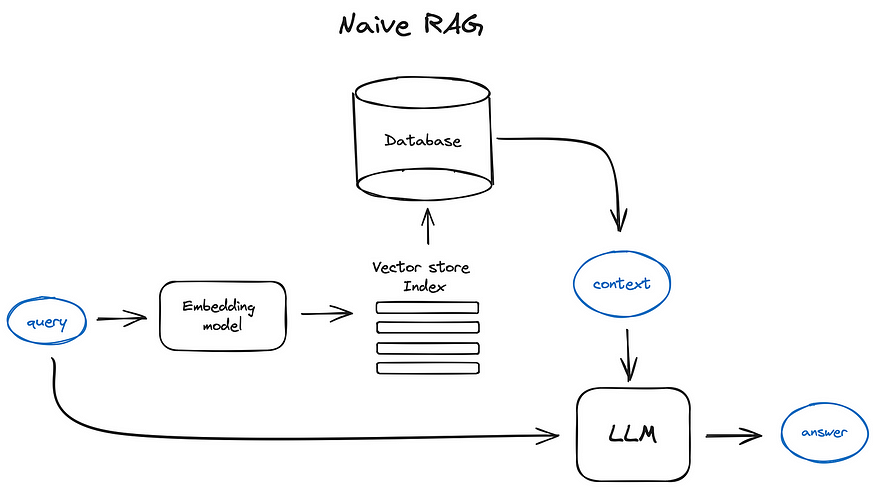
\includegraphics[width=\linewidth]{images/native diagrammme llm.png}
		\captionof{figure}{Phases de la Génération du Contexte}
\end{minipage}
\paragraph{}
Pour combler cet écart sémantique, nous utilisons un processus de recherche en deux étapes qui exploite la capacité des modèles de langage de grande taille (LLM) à faire le lien entre ces différents domaines. Nous commençons par solliciter GPT-3.5-turbo (Brown et al., 2020) afin de générer une description de cours « idéale », qui correspondrait parfaitement aux intérêts et au niveau de l’étudiant. Cette description idéalisée sert ensuite de vecteur de requête plus efficace pour notre système de recherche basé sur les embeddings, car elle traduit l’expression en langage naturel des intérêts de l’étudiant en un langage académique structuré, typique des descriptions de cours.

En alignant les caractéristiques linguistiques de la requête avec celles des documents cibles avant de calculer les embeddings, nous veillons à ce que la recherche vectorielle capte une pertinence sémantique réelle, au lieu d’être perturbée par des différences de style ou de structure linguistique. Nous utilisons GPT-3.5-turbo en raison de sa rapidité, car les capacités plus avancées des modèles plus grands ne sont pas nécessaires pour cette tâche de génération.

Concrètement, le processus de recherche adopte une approche en deux étapes, décrite dans les Algorithmes 1 et 2, pour identifier les 50 cours les plus pertinents sur le plan sémantique. Ces cours sélectionnés sont ensuite regroupés dans une chaîne de contexte structurée, composée des identifiants des cours et de leurs descriptions respectives. Cette chaîne de contexte constitue la base de l’étape de recommandation.

\section{Recommandation}

Après avoir généré un contexte filtré des cours les plus pertinents sur le plan sémantique, le système utilise le modèle \texttt{ollama/llama3.2} pour formuler la recommandation finale. Nous tirons parti des capacités de raisonnement avancées de LLaMA 3.2 pour évaluer plus efficacement l'interaction complexe entre les intérêts des étudiants, le contenu des cours et les trajectoires éducatives.

L’ingénierie des invites (\textit{prompt engineering}) pour la génération des recommandations repose sur trois objectifs principaux :
\begin{itemize}
    \item maintenir la qualité des recommandations,
    \item assurer la fiabilité du système,
    \item fournir des informations exploitables.
\end{itemize}

Afin de garantir une cohérence maximale entre les réponses, nous fixons le paramètre \texttt{temperature} à 0, bien que des variations notables puissent subsister dans les cas de requêtes ouvertes --- un comportement que nous discutons dans la section des résultats.

Le système retourne un ensemble de dix recommandations de cours, présentées en format Markdown pour une lisibilité optimale. Chaque recommandation comprend :
\begin{itemize}
    \item l’identifiant du cours,
    \item une justification courte et ciblée expliquant la pertinence du cours par rapport au profil de l’étudiant,
    \item une évaluation du niveau de confiance (\textit{élevé}, \textit{moyen} ou \textit{faible}).
\end{itemize}

Ce format structuré permet de concilier exhaustivité et clarté --- dix options offrent une diversité suffisante tout en restant faciles à analyser. Les justifications apportent un contexte décisionnel concret pour aider l’étudiant à faire un choix éclairé. Des liens vers des informations supplémentaires sur chaque cours seront ajoutés avant le déploiement officiel.

Pour garantir l’intégrité des recommandations et prévenir toute forme de désinformation, plusieurs contraintes sont imposées au système :
\begin{itemize}
    \item Il ne fournit pas de conseils académiques généraux,
    \item Il ne discute pas des prérequis absents des descriptions de cours,
    \item Il ne recommande pas de cours hors contexte.
\end{itemize}

Ces règles assurent que le système reste strictement un moteur de recommandation de cours basé sur le contexte fourni, sans se substituer à un conseiller académique humain.
